\chapter{Diffusion measurements in the CERN LHC}
\noindent\textsf{The content of this chapter, with the due adaptations, has resulted in the proceedings by C.\ E.\ Montanari, A.\ Bazzani, M.\ Giovannozzi, A.\ A.\ Gorzawski, and S.\ Redaelli \textit{\citetitle{montanari:ipac22-mopost043}}, which were presented as a poster at IPAC'22 in June 2022~(Ref.~\cite{montanari:ipac22-mopost043}).}

\section{The LHC collimation system}

The layout of the LHC~\cite{Bruning:782076} can be summarized in a geometrical scheme composed by 8 straight Insertion Regions (IRs) and 8 circular arc segments. A simple scheme of this layout is reported in Fig.~\ref{fig:lhc_layout}. Within this circular scheme, the main particle physics experiments are located in IR1, IR2, IR5, and IR8, namely, ATLAS~\cite{TheATLASCollaboration_2008}, ALICE~\cite{Alessandro:879894}, CMS~\cite{Chatrchyan:1129810}, and LHCb~\cite{Alves:1129809}. In these four IRs, the two beams intersect and interact in what is referred to as an Interaction Point (IP). The RF cavities for accelerating the beams are in IR4 and IR6 hosts the beam extraction system. Finally, IR3 and IR7 are dedicated, respectively, to the longitudinal and transverse collimation system.

\begin{figure}[htp]
    \centering
    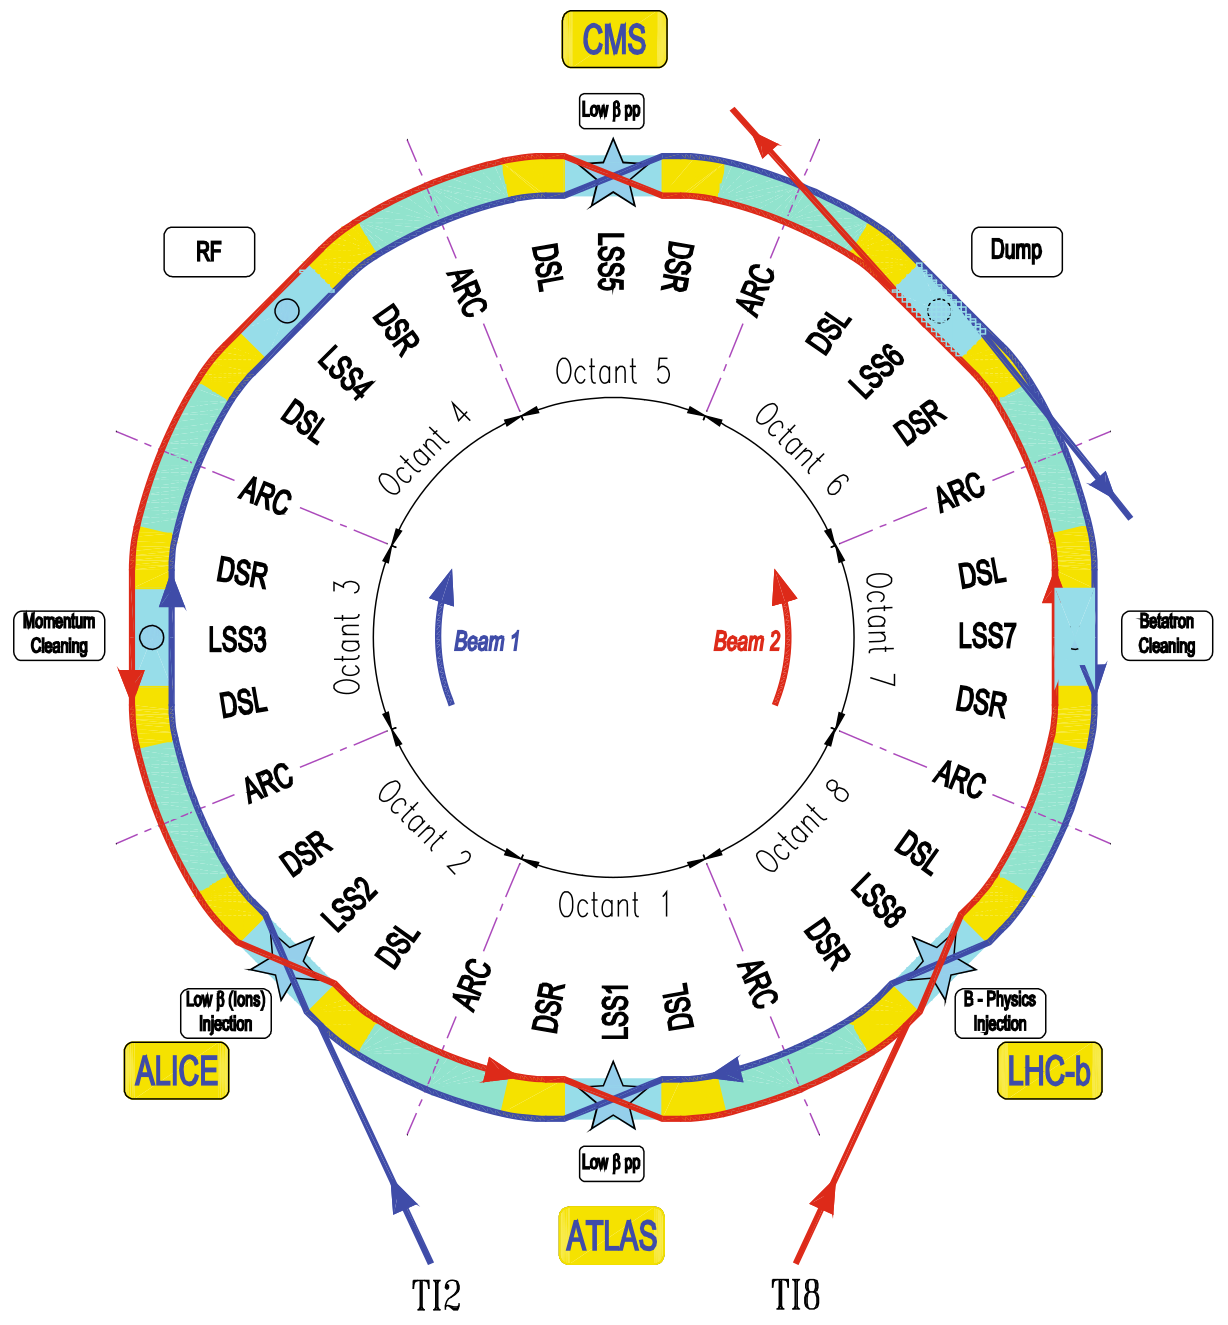
\includegraphics[width=0.75\textwidth]{5_Diffusion_measurement_LHC/figs/layout.png}
    \caption{Layout of the LHC. The ring follows a visible eightfold symmetry. Each octant hosts a Long Straight Sector (LSS) surrounded by two Dispersion Suppressor regions (DSR and DSL). Each octant is connected by a long arc (ARC). (From Ref.~\cite{Bruning:782076})}
    \label{fig:lhc_layout}
\end{figure}

The LHC collimation system is a fundamental component to the machine operation and security~\cite{1590664, Assmann:972336}. It has multiple functions, such as cleaning the beam halo, protecting the machine for expected and anomalous losses~\cite{BRUCE201719}, and reducing the background noise at the experiments IPs~\cite{Bruce:1646958, Bruce:2686581}.

The collimation system counts more than 120 individual collimators. The majority of these collimators are movable devices constituted by two movable jaws made of solid material, which can be brought at different distances from the circulating beam~\cite{Bertarelli:794628}. These jaws are straight and parallel to the beam and have a tapering on both ending sides, along the axis of the beam. The distance between the start and end of the tapering, where the jaw material is straight, is referred to as the active length of the collimator. Some photos and schemes of these LHC collimators are reported in Fig.~\ref{fig:collimator_pics}.

\begin{figure}[htp]
    \centering
    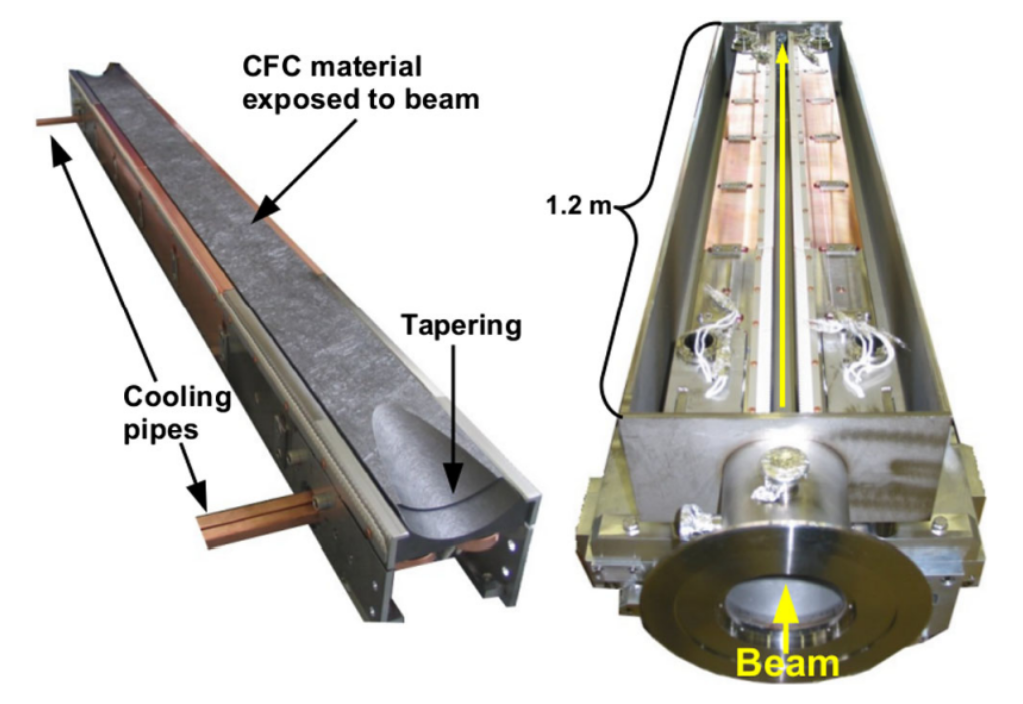
\includegraphics[width=0.75\textwidth]{5_Diffusion_measurement_LHC/figs/collimator_pics.png}
    \caption{Left picture, jaw of a secondary collimator, made of carbon-fiber composite (CFC) and water cooled through copper pipes. Right picture, two collimator jaws are installed in a collimator tank. (From Ref.~\cite{bruce2014simulations})}
    \label{fig:collimator_pics}
\end{figure}

At IR7, where transversal collimators are located, we have an effective cleaning stage of halo particles that happen to have and excessively large betatron oscillation. In this precise region, the magnetic lattice optics is configured so that we can observe a maximum separation for such particles (i.e.\ the $\beta$ function for this region is kept particularly large). A cleaning of particles with large longitudinal deviations happens instead in IR3, where additional horizontal dispersion is introduced to translate the momentum defect of the halo particles into a physical trajectory deviation.

In IR7, there are 3 sets of collimators covering the horizontal, vertical and skew planes. In IR3, the dispersion is only in the horizontal and only one set of collimators is installed.

To safely clean the beam halo without damaging the magnets or other components of the machine, the LHC collimation systems follows a multi-stage process. This multi-stage process consists of a \textit{hierarchy} of individual collimators with the purpose to progressively clean and channel the particle loss. A scheme of this hierarchy is presented in Fig.~\ref{fig:collimator_hierarchy}.

\begin{figure}[htp]
    \centering
    \def\svgwidth{1.0\columnwidth}
    \import{5_Diffusion_measurement_LHC/figs}{hierarchy.pdf_tex}
    \caption{Scheme of the multistage collimation system inside the LHC. The hierarchy includes primary (TCP), secondary (TCSG) and tertiary (TCT) collimators and shower absorbers (TCLA). Particles from the primary halo collide with the TCP and are scattered to the TCSGs. The hadronic showers coming from the TCSGs are finally absorbed by the TCLAs, and TCTs are in place to protect the aperture bottlenecks. Part of the secondary halo interacts with the ionization chambers of the BLMs, and provide an indirect measurement of the primary halo. (Scheme based on Ref.~\cite{Hermes:2241364})}
    \label{fig:collimator_hierarchy}
\end{figure}

The primary collimators, which are also referred to as \textit{Target Collimator Primary} (TCP), are the ones placed the closest to the beam and form the first stage of collimation. The purpose of this first collimation stage is to intercept and dispose of beam halo particles, i.e.\ it is the stage at which the beam halo actually gets intercepted above a certain threshold. When interacting with the primary collimators matter, the particles may exhibit various scattering behaviours ranging from acquiring an angular kick, to depositing energy, and producing secondary particles. 

These particles, scattered by the TCPs, form the secondary halo, which is then tackled by the secondary collimators, \textit{Target Collimator Secondary-Graphite} (TCSG). The particles leaving the collimator finally form the tertiary halo, which finally interacts with the active absorbers, \textit{Target Collimator Long Absorber} (TCLA), which are installed downstream of the TCSGs, and \textit{Target Collimator Tertiarys} (TCTs), which make up a final third collimation stage for local protection for the aperture bottlenecks in the machine.

The secondary particle showers represent the point of observation for measuring the amount of particles lost at the TCPs. To quantify this amount, the LHC is equipped with multiple ionization chambers, with constitute the Beam Loss Monitor (BLM) system~\cite{blmSystem1, blmSystem2}. The charged particles traversing the ionization chambers finally provide a measure of \SI{}{Gy \per s}, which can be converted into a corresponding measure of \SI{}{p \per s} lost using a calibration factor, evaluated via controlled collimator-induced losses~\cite{arek}, which are also quantified in parallel by the \textit{DC Beam Current Transformer} (BCT) system~\cite{Denard:1213275}. A picture of an LHC BLM is presented in Fig.~\ref{fig:blm}. This calibrated BLM data is the precise loss signal that we finally expect to use for reconstructing the diffusion behaviour in the transverse plane.

\begin{figure}[htp]
    \centering
    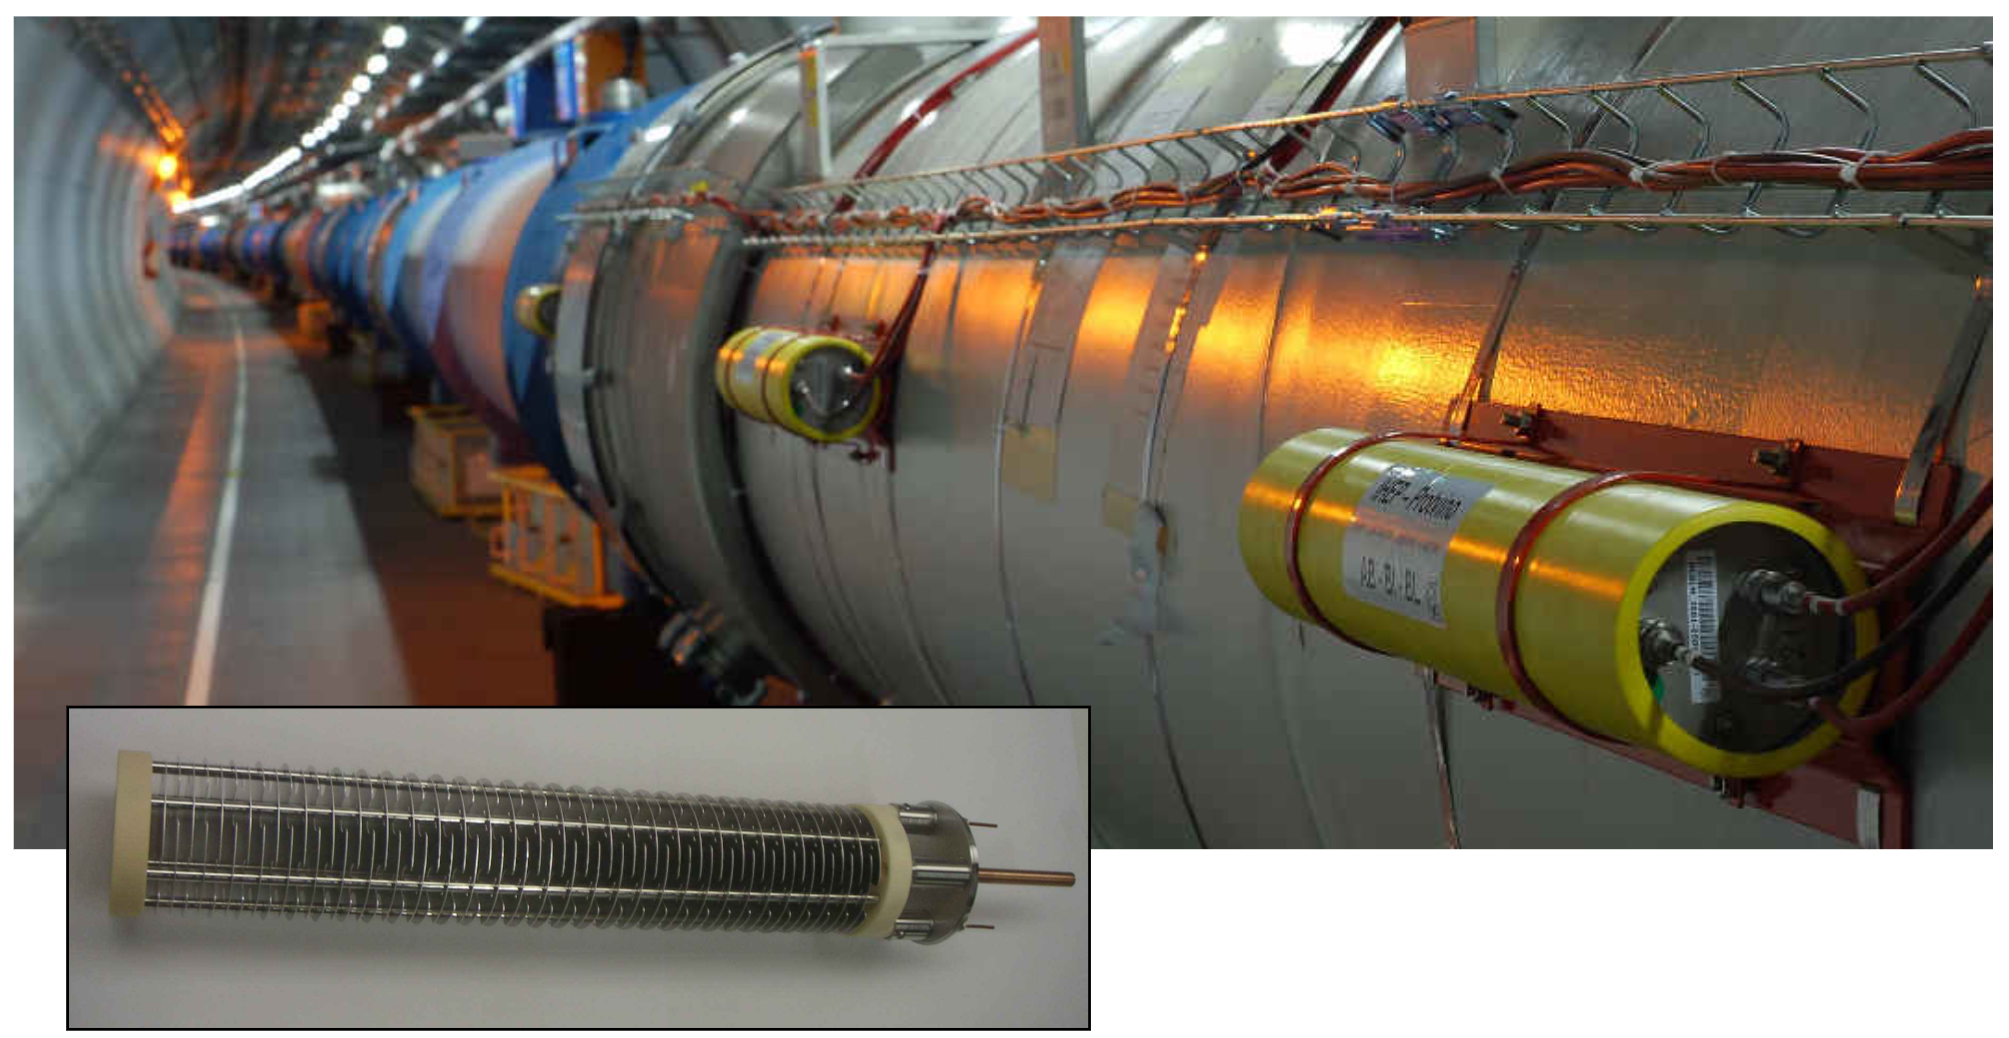
\includegraphics[width=0.75\textwidth]{5_Diffusion_measurement_LHC/figs/blm.png}
    \caption{Top picture, ionization chambers of the LHC BLM system, mounted on the side of the LHC Magnets. Bottom picture, inner structure of a BLM ionization chamber. (From Ref.~\cite{blmonline})}
    \label{fig:blm}
\end{figure}


%
\section{Analysis of experimental data}
%

Between 2016 and 2018, collimator scans were performed at the CERN LHC with physics beams at \SI{6.5}{TeV}~\cite{PhysRevAccelBeams.23.044802}. During these scans, one of the jaws of the IR7 primary collimators was moved inwards and outwards in small steps, starting at $~5\sigma_\text{nom}$, where the nominal sigma value $\sigma_\text{nom}$ is evaluated for a nominal emittance $\varepsilon_\text{nom} = 3.5$.

The scan was performed after executing a beam-based alignment~\cite{valentino2012semiautomatic} of the collimator, which is a procedure in which the TCP jaws are progressively set closer to the beam until the halo is touched. By performing such procedure, one is sure that the collimator gap centre is precisely around the local closed orbit.

The measurement is performed with the local beam loss monitoring (BLM) system, and is provided in unit of \SI{}{Gy \per s} with \SI{1}{Hz} sampling rate, processed over different running sums (RS)~\cite{Bruning:782076}. In Fig.~\ref{fig:raw_data} we present the data gathered during fill 6052 of type RS06, i.e.\ sampling the maximum spike measured by the BLM over a time window of \SI{10.24}{ms}. The collimator jaw positions here is reported in millimetres from the nominal centre of the beam.

\begin{figure}[htp]
    \centering
    % 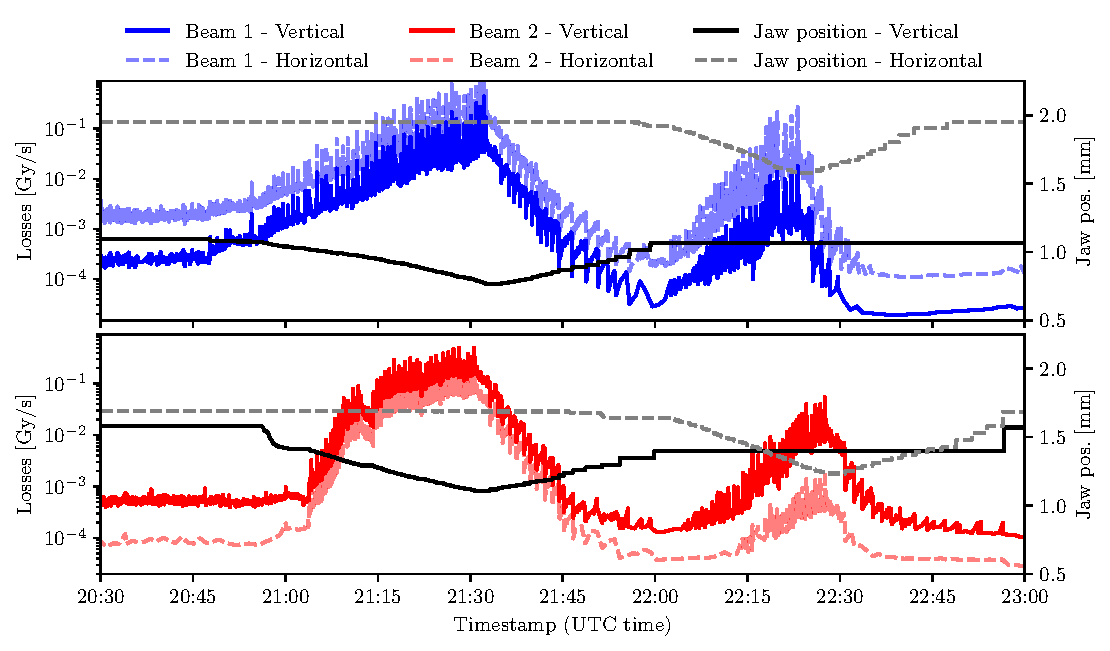
\includegraphics[trim={0 2.5mm 0 4mm}, clip, width=\textwidth]{5_Diffusion_measurement_LHC/figs/raw.pdf}
    \caption{Beam loss data from the BLM monitor at RS06 (i.e.\ the maximum spike over a time window of \SI{10.24}{ms}) for Beam1 and Beam2, and positions of IR7 TCP jaws measured in the vertical and horizontal plane for the collimator scans carried out in fill 6052. The data acquired represent a complete collimator scan on both planes. (Data from Ref.~\cite{PhysRevAccelBeams.23.044802})}
    \label{fig:raw_data}
\end{figure}

One can see how the IR7 TCPs vertical and horizontal jaws of both Beam1 and Beam2 were used to perform a so-called collimator scan of the beam halo, performing a train of inward steps, with pauses of a few seconds between the steps, followed up by a train of outward steps, with pauses ranging from $\sim30$ seconds to almost two minutes between steps.

It should be stressed that these older collimator scans were not performed using the optimal protocol, proposed in the previous Chapter, as complete inward scans, followed by outward scans, were used instead of a sequence of in/out steps. Moreover, the jaw movements were not always performed to allow enough time for the system to relax to its equilibrium state. This can be observed from the fact that, between most outward steps, the loss signal still has a consistent positive first derivative when the next collimator outward step is performed, suggesting that a consistent recovery current process was still ongoing when the jaw was moved.

Due to these two differences in the measurement protocol used during the collimation scan, some of the working hypothesis made in the previous Chapter, which ultimately enable the reconstruction of $D(I)$ via the fitting of the normalized recovery current, may not hold. Most specifically, we do lack the upper bound for reconstructing the global current, and we can not be sure that the beam tail distribution after an outward step follows Eq.~\eqref{eq:outward_difference}.

To tackle these characteristics and shortcomings of the data, we had to consider only a subset of the data and modify some of the elements of the fitting procedure. 

To address the lack of alternating jaw movements, we selected a region of interest (ROI) in which many outward steps were performed with almost regular sampling, with loss signals exhibiting the features we expect to see from a recovery current. This decision is motivated by the fact that the simulation study presented in the previous Chapter shows how recovery currents induced by outward steps are much more reliable for reconstruction purposes than the ones induced by inward steps. In Fig.~\ref{fig:first} we present the portion of the data collected in fill 6052 which we finally selected. Unfortunately, only the scraping performed in the vertical plane meets our quality requirements for applying the fitting of our diffusive model.

\begin{figure}[htp]
    \centering
    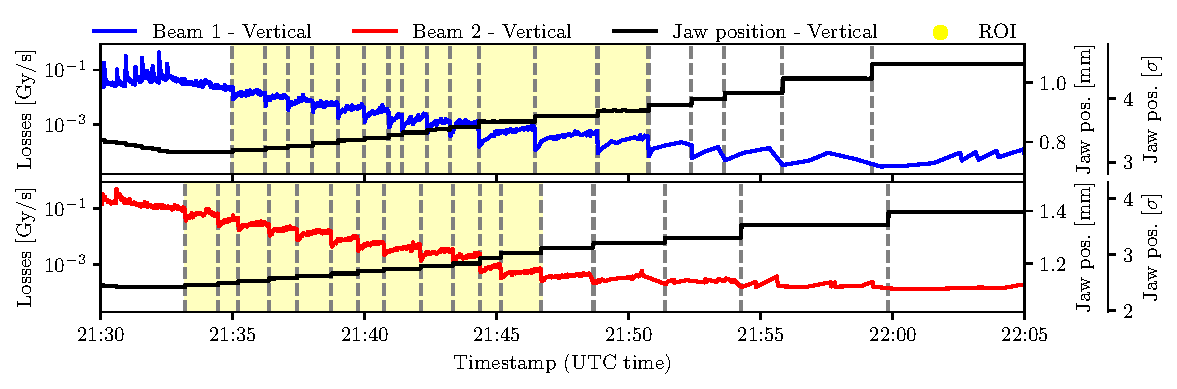
\includegraphics[trim={0 2.5mm 0 4mm}, clip, width=\textwidth]{5_Diffusion_measurement_LHC/figs/first.pdf}
    \caption{Selected data from fill 6052 (i.e.\ Fig.~\ref{fig:raw_data}). The data shown correspond to outward jaw movements in the vertical plane. The yellow-marked region of interest (ROI) represents a subset of data meeting our quality requirements for applying the fitting of our diffusive model. (Data from Ref.~\cite{PhysRevAccelBeams.23.044802})}
    \label{fig:first}
\end{figure}


The measured collimator jaw position is converted to measured beam sigma units using the nominal optical parameters and the measured value of the beam emittance, taking into account the position of the beam centre. To convert the \SI{}{Gy \per s} units of the BLM signal to \SI{}{protons \per s}, we used a calibration factor $F$~\cite{arek} dependent on the TCP jaw position. This calibration factor $F$ is calculated from the BLM loss data and the intensity lost recorded by the BCTs during the collimator steps. The coefficient reads 
\begin{equation}
    F = \left(-9.0\times10^{-14}\sigma + 6.2\times10^{-13}\right)^{-1} \,.
\end{equation}

To reconstruct an estimate global current $J_\text{eq}^{\text{est}}(t)$, without the upper bound given by the alternating inward steps, with a single CSI passing through the terminating points of the sequence of outward recovery currents. This fundamental CSI has been multiplied by a constant term to represent different possible levels of partial recovery of $J_\mathrm{R}(t)$. This is needed because the jaw movements were not always performed to allow enough time for the system to relax to its equilibrium state. This procedure is shown in Fig.~\ref{fig:second}.

%
\begin{figure}
    \centering
    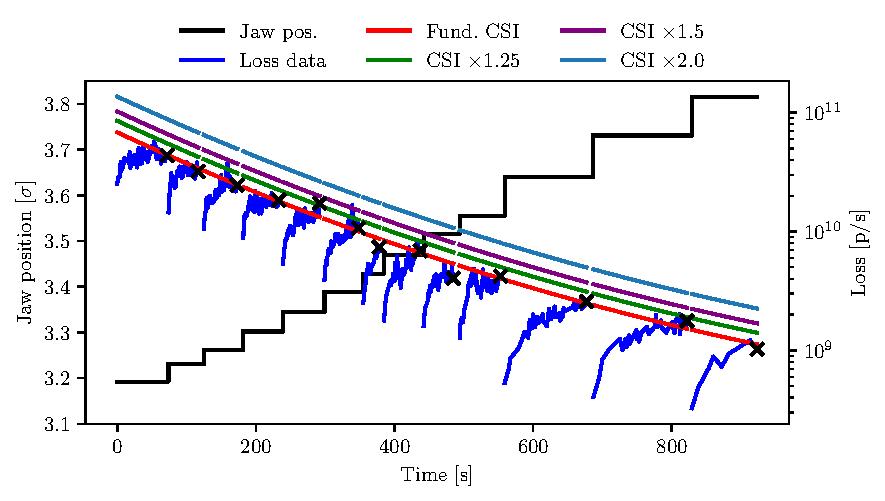
\includegraphics[trim={0 2.5mm 0 3mm}, clip, width=\columnwidth]{5_Diffusion_measurement_LHC/figs/second_bis.pdf}
    \caption{Possible estimates of $J_\mathrm{eq}(t)$ for Beam1 data. An initial estimate is made starting from a Cubic Spline Interpolation (CSI) with positive second derivative passing through the end points of the measured recovery currents (red line). The various curves are obtained by multiplying the fundamental CSI by a constant term, and represent estimates of the partial recovery currents. The multiplicative constant considered is reported in the plot legend.}
    \label{fig:second}
\end{figure}
%

To cope with the rapid sequence of jaw movements, we replace the integral terms in Eq.~\eqref{eq:outward_difference_approx} with the approximation
\begin{equation}
    \rho_{\mathrm{app}}^{*}(I)= \begin{cases} -M & \text { if } I\leq I_{\mathrm{a}}\\ -\left(\frac{I_{\mathrm{a}}^{\prime }-I}{I_{\mathrm{a}}^{ \prime}-I_{\mathrm{a}}}\right) M & \text { if } I>I_{\mathrm{a}} \, , \end{cases} 
    \label{eq:approximated_distribution_beam}
\end{equation}
where $M$ is a constant fixed for each jaw movement that represents an unknown amount of out-of-equilibrium distribution.
A scan is performed on different combinations of CSI and $M$ values while keeping track of $\chi^2$ achieved by the fitting routine that determines the values of the model parameters $\kappa, I_\ast$. The result of this procedure is shown in Figs.~\ref{fig:fourth} and~\ref{fig:fifth}, where one can observe the existence of an optimal configuration of parameters and the good reconstruction performance achieved by such a configuration. The optimal fit results for Beam~1 and Beam~2 data are reported in Table~\ref{tab:fit_results}.

\begin{figure}
    \centering
    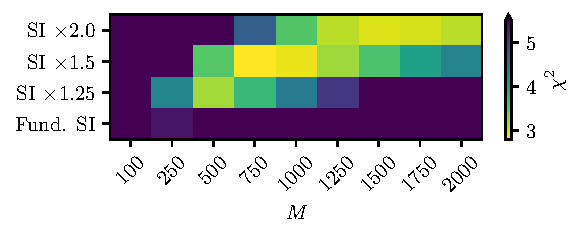
\includegraphics[trim={0 2.5mm 0 1.5mm}, clip, width=0.98\columnwidth]{5_Diffusion_measurement_LHC/figs/fourth.pdf}
    \caption{Fit performance of $\kappa$ and $I_\ast$ for Beam1 data, using different combinations of CSI multiplicative constants and values of $M$ for Eq.~\eqref{eq:approximated_distribution_beam}. The colormap shows the existence of an optimal pair of values at (CSI $\times 1.5$, $750$).}
    \label{fig:fourth}
\end{figure}
%
\begin{table}[htb]
    \centering
    \caption{Results of the fit procedure, along with corresponding setup obtained for the CSI multiplicative constant and $M$ value for \eqref{eq:approximated_distribution_beam}.}
    \begin{tabular}{lcccc}
        \toprule
        Beam / Plane & CSI & $M$ & $\kappa$ & $I_\ast\ [\sigma]$ \\
        \midrule
        Beam~1 / V & $\times1.5$ & $750$ & $0.59\pm0.03$ & $21\pm2$ \\
        Beam~2 / V & $\times1.5$ & $1000$ & $0.85\pm0.02$ & $39\pm8$ \\
        \bottomrule
    \end{tabular}
    \label{tab:fit_results}
\end{table}
%

Note that the values reported in~\cite{bazzani2020diffusion}, namely $\kappa=0.33 $ and $I_\ast \simeq 21$, were obtained for Beam~2 and considering the diffusion in the vertical plane. It should be stressed that these previous measurements were performed with isolated bunches, whereas in the beam measurements analysed here, beam-beam effects were present. 

\begin{figure}[htb]
    \centering
    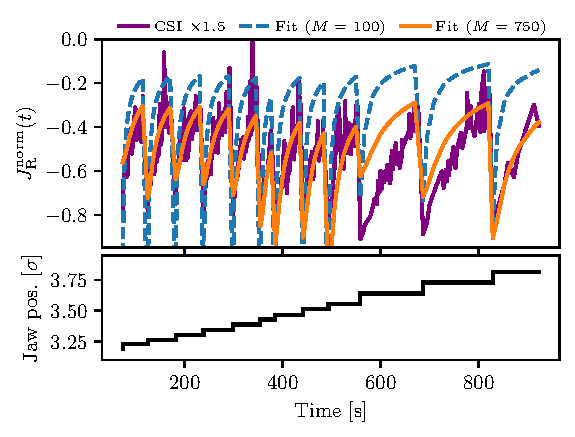
\includegraphics[trim={0 2.5mm 0 3mm}, clip, width=0.95\columnwidth]{5_Diffusion_measurement_LHC/figs/fifth.pdf}
    \caption{Fit results for Beam~1 data for two $M$ values. The optimal value (orange) outperforms a lower value (blue).}
    \label{fig:fifth}
\end{figure}
%
\section{Final remarks}
%
A non-linear diffusive model based on Nekhoroshev theorem was used to reconstruct available beam loss data obtained at the  LHC from collimator scans. The differences between the approach used to gather the data and the optimal one suggested by our recent numerical studies required adaptation of some of the key elements of our fitting procedure. Eventually, this led to good reconstruction performances and promising insights into the global diffusive behaviour of the LHC beam halo.

Future research will focus on acquiring beam data using the proposed optimised experimental method to characterise more accurately the presence of nonlinear diffusive behaviour. The new datasets might also be used to perform comparisons between the newly proposed collimator scan method for the Nekhoroshev-based diffusive model and the previous approach based on the linearisation of the diffusion coefficient around a given jaw position.
